\documentclass[sigconf,nonacm]{acmart}

\usepackage{lmodern}
\usepackage{booktabs}
\usepackage{amsmath}
\usepackage{amsthm}
\usepackage{graphicx}
\usepackage{listings}
\usepackage{xcolor}
\usepackage{pifont}
\newcommand{\cmark}{\textcolor{green!55!black}{\ding{51}}}
\newcommand{\xmark}{\textcolor{red!70!black}{\ding{55}}}

\theoremstyle{definition}
\newtheorem{definition}{Definition}

\sloppy
\emergencystretch=3em

\title[GPU-Accelerated Continuous Subgraph Matching]{GPU-Accelerated Continuous Subgraph Matching: Why BFS Beats DFS on the SIMT Architecture}

\author{Haibin Lai}
\affiliation{%
  \institution{Southern University of Science and Technology}
  \city{Shenzhen}
  \country{China}
}
\email{12211612@mail.sustech.edu.cn}

\author{Ziheng Wang}
\affiliation{%
  \institution{Southern University of Science and Technology}
  \city{Shenzhen}
  \country{China}
}
\email{12310401@mail.sustech.edu.cn}

\author{Rongchuan Li}
\affiliation{%
  \institution{Southern University of Science and Technology}
  \city{Shenzhen}
  \country{China}
}
\email{12211402@mail.sustech.edu.cn}

\begin{document}

\begin{abstract}
Continuous Subgraph Matching (CSM) enumerates, for a small query graph, all of its embeddings under a stream of edge updates to a large data graph. ParaCOSM~\cite{paracosm2025} demonstrated two-level parallelism on multi-core CPUs. We extend ParaCOSM to the GPU and report two findings. First, on the dense Amazon (AZ) graph and an 8-vertex query workload, a level-synchronous BFS pipeline accelerates four of five state-of-the-art CSM algorithms (\textsc{NewSP}, \textsc{TurboFlux}, \textsc{GraphFlow}, \textsc{SymBi}) by a median of $25\times$--$51\times$ over a single-threaded CPU baseline. Second, the BFS choice is not incidental: a depth-first GPU implementation suffers from stack-pointer divergence, hub-vertex load imbalance, and unstructured memory access, and is dominated on every algorithm-query pair we tried. We characterize the search-tree growth that underpins both observations, identify a buffer-overflow regime that causes performance to collapse on the highly skewed LiveJournal (LJ) graph, and discuss several work-balanced and streaming improvements that target the observed bottlenecks.
\end{abstract}

\keywords{Continuous subgraph matching, GPU acceleration, BFS vs DFS, SIMT, graph algorithms}

\maketitle

% ============================================================================
\section{Introduction}
% ============================================================================
Continuous Subgraph Matching (CSM) is the task of maintaining, in real time, all embeddings of a small query graph $q$ in a large data graph $G$ that is updated by a stream of edge insertions and deletions. CSM is the kernel of stream graph analytics in financial risk control on transaction graphs~\cite{zhang2024bg3}, real-time recommendation on social-interaction streams~\cite{gupta2014twitter}, and graph-based network-security and botnet monitoring~\cite{lagraa2024network}. Recent algorithmic progress has produced several state-of-the-art CPU systems---\textsc{GraphFlow}~\cite{graphflow}, \textsc{TurboFlux}~\cite{turboflux}, \textsc{SymBi}~\cite{rapids-symbi}, \textsc{CaLiG}~\cite{calig}, and \textsc{NewSP}~\cite{newsp}---each with a distinct trade-off between filtering, indexing, and search cost.

ParaCOSM~\cite{paracosm2025} consolidated these algorithms behind a common executor and added two layers of CPU parallelism: \emph{inner-update} parallelism for searches launched by a single update, and \emph{inter-update} parallelism over disjoint safe updates. The CPU implementation scales well at low thread counts, but the per-update search itself remains the bottleneck on dense workloads.

This report describes a GPU port of ParaCOSM's search and classification stages. The natural design question is whether to reuse the CPU implementation's depth-first recursion, parallelizing across many independent search trees on the GPU, as cuTS~\cite{xiang2021cuts}, GCSM~\cite{wei2024gcsm}, and the GPU batch-dynamic system of Qiu~et~al.~\cite{qiu2024gpubatch} do, or to switch to a level-synchronous breadth-first pipeline that is closer to GPU graph-traversal kernels~\cite{merrill2015hpcgraph} and the partition-balanced design of Jupiter~\cite{lin2025jupiter}. We report on both alternatives and summarize three contributions:

\begin{enumerate}
    \item \textbf{A GPU-BFS pipeline} (\texttt{gpu\_bfs\_versioned}) for the unsafe-update search of all five CSM algorithms, with a versioned timestamp protocol that lets multiple updates share a single GPU search.
    \item \textbf{An empirical case for BFS over DFS on the GPU.} On AZ at 8-vertex queries, BFS-versioned achieves a median speedup of $51.1\times$, $49.5\times$, $46.5\times$, $25.3\times$, and $21.7\times$ on \textsc{NewSP}, \textsc{TurboFlux}, \textsc{GraphFlow}, \textsc{SymBi}, and \textsc{CaLiG} respectively, while the DFS variant is consistently dominated.
    \item \textbf{A characterization of the boundary of GPU benefit.} On the very sparse and skewed LiveJournal (LJ) graph, the BFS frontier explodes into the $10^{10}$-match regime and the partial-match buffer overflows; we identify the bottleneck and outline three concrete improvements.
\end{enumerate}

% ============================================================================
\section{Background and System}
% ============================================================================

\subsection{Formal Definitions}
\label{sec:defs}

\begin{figure}[t]
\centering
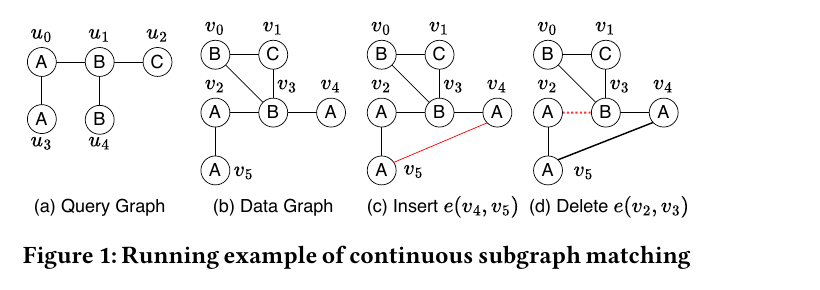
\includegraphics[width=\columnwidth]{figures/csm_running_example.png}
\caption{Running example of continuous subgraph matching, reproduced from ParaCOSM~\cite{paracosm2025} (Fig.~1).}
\label{fig:csm-running}
\end{figure}

We adopt the formalism of ParaCOSM~\cite{paracosm2025}. Throughout, $g=(V,E)$ denotes a labeled undirected graph with vertex- and edge-labeling functions $L_V\!:\!V\!\to\!\Sigma_V$ and $L_E\!:\!E\!\to\!\Sigma_E$ (jointly written $L$); $N(u)$ and $d(u)\!=\!|N(u)|$ are the neighbor set and degree of $u$. We write $G$ for the data graph and $Q$ for the query graph.

\begin{definition}[Subgraph match]
A \emph{match} of $Q$ in $G$ is an injection $M\!:\!V(Q)\!\to\!V(G)$ such that
\begin{enumerate}
\item[(i)]   $L(u)=L(M(u))$ for every $u\in V(Q)$;
\item[(ii)]  $L(e(u,u'))=L(e(M(u),M(u')))$ for every $e(u,u')\in E(Q)$;
\item[(iii)] $e(M(u),M(u'))\in E(G)$ for every $e(u,u')\in E(Q)$.
\end{enumerate}
We denote the set of all such matches by $\mathcal{M}$.
\end{definition}

\begin{definition}[Graph stream]
The data graph evolves under a sequence
$\Delta\mathcal{G}=(\Delta G_1,\Delta G_2,\dots)$ of single-element updates,
each of the form $\Delta G=(\pm,\,e/v)$ — i.e., insertion or deletion of one
edge or vertex. Applying $\Delta G$ to $G$ yields $G'$.
\end{definition}

\begin{definition}[CSM problem~\cite{paracosm2025}]
Given $G$, $Q$, and $\Delta\mathcal{G}$, CSM reports, for every $\Delta G\in\Delta\mathcal{G}$, the \emph{incremental match set}
$\Delta\mathcal{M} = \mathcal{M}'\!\setminus\!\mathcal{M}\;\cup\;\mathcal{M}\!\setminus\!\mathcal{M}'$,
i.e., the matches that newly appear or expire as a result of $\Delta G$.
\end{definition}

\begin{definition}[Compatible set]
For a partial mapping $\phi\!:\!V'_Q\!\to\!V'_G$ that satisfies the matching constraints on the matched-so-far vertices, the \emph{compatible set} of an unmatched query vertex $u\in V_Q\!\setminus\!V'_Q$ is
$C(u,\phi)=\{v\in V_G\!\setminus\!V'_G \mid \phi\cup\{(u,v)\}\text{ remains valid}\}.$
\end{definition}

\subsection{The Two-Stage Model}

\begin{figure}[t]
\centering
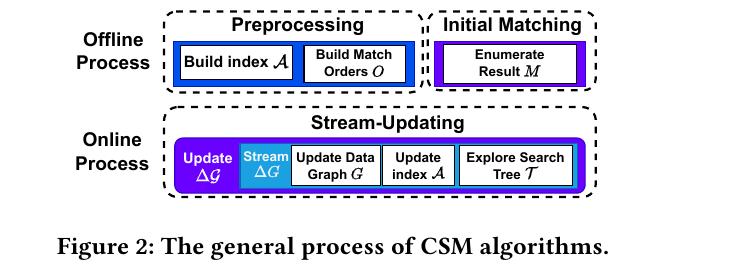
\includegraphics[width=\columnwidth]{figures/csm_general_workflow.png}
\caption{General two-stage workflow of CSM algorithms (offline + online), reproduced from ParaCOSM~\cite{paracosm2025} (Fig.~2).}
\label{fig:csm-workflow}
\end{figure}

Following the survey of Sun~et~al.~\cite{calig} and the unified view of ParaCOSM, every CSM algorithm decomposes into (see Fig.~\ref{fig:csm-workflow}):

\paragraph{Offline stage.} Build an auxiliary data structure $\mathcal{A}$ (DCS for SymBi, candidate-set index for CaLiG, DAG order for TurboFlux, none for GraphFlow, CPT/EXP order for NewSP), pick a matching order $\mathcal{O}$, and (optionally) compute initial matches $\mathcal{M}_0$.

\paragraph{Online stage.} For each $\Delta G$:
\begin{enumerate}
  \item update the data graph and the auxiliary structure: $\mathcal{A}\!\leftarrow\!\textsc{Update}\_\textsc{ADS}(Q,\mathcal{A},\Delta G)$;
  \item build the search tree $\mathcal{T}$ rooted at the inserted/deleted edge $e$ following $\mathcal{O}$;
  \item enumerate $\Delta\mathcal{M}$ by traversing $\mathcal{T}$. The traversal expands a partial match $M$ by selecting the next query vertex $u$, computing $C(u,M)$, and recursing into each valid extension.
\end{enumerate}

\subsection{Safe vs. Unsafe Updates}
\label{sec:safe}
ParaCOSM observes that, on real workloads, more than $98.4\%$ of edge updates do \emph{not} change $\mathcal{M}$. It calls these \emph{safe}; the remainder are \emph{unsafe}. Concretely, an update is classified \texttt{unsafe} if any of the following triggers fires: (i) \emph{label} filter — its endpoint labels match some query edge; (ii) \emph{degree} filter — both endpoints reach the degree threshold of a query vertex; (iii) \emph{candidate} filter — it perturbs $\mathcal{A}$ in a way that may invalidate other concurrent matches.

Safe updates can be batched and applied in parallel to $G$ alone; unsafe updates must each launch a search. The GPU work in this report targets the per-unsafe-update \emph{search}, which dominates wall time even after the safe-update fast path is taken.

\subsection{What This Report Adds: A GPU Back-End}

\begin{figure}[t]
\centering
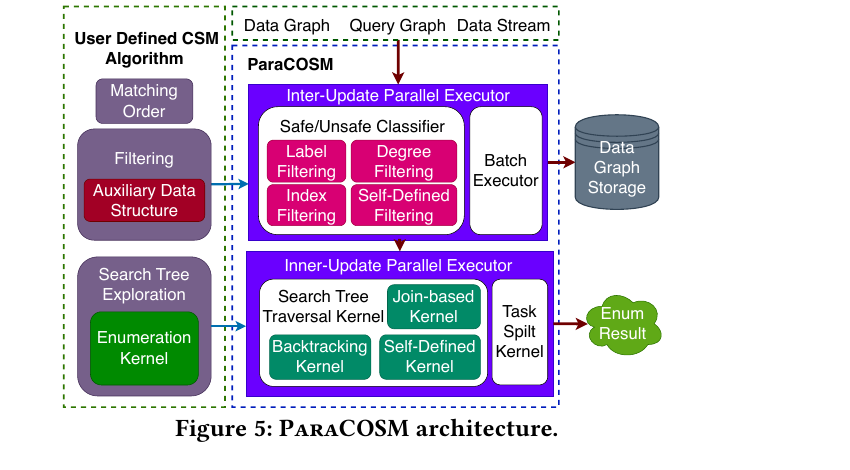
\includegraphics[width=\columnwidth]{figures/csm_paracosm_arch.png}
\caption{ParaCOSM architecture (reproduced from~\cite{paracosm2025}, Fig.~5). Our GPU back-end replaces the inter-update and inner-update parallel executors with CUDA kernels while keeping the user-defined hooks (matching order, filtering, search-tree exploration) unchanged.}
\label{fig:paracosm-arch}
\end{figure}

On top of ParaCOSM's CPU runtime (Fig.~\ref{fig:paracosm-arch}), we add four GPU modules; each one implements one of the boxes in the online loop above:

\begin{itemize}
    \item \texttt{gpu\_classifier} (mode \texttt{-m gpu}). Implements the safe/unsafe classifier of \S\ref{sec:safe} on the device, fusing label, degree, and candidate filters into one kernel.
    \item \texttt{gpu\_candidate\_filter} (auto, PFM2). Computes $C(u,\phi)$ for adjacent query vertices in parallel.
    \item \texttt{gpu\_search} (mode \texttt{-m gpu\_all}). DFS-style traversal of $\mathcal{T}$; one thread per root, with a per-thread stack.
    \item \texttt{gpu\_bfs\_search} (modes \texttt{-m gpu\_bfs} and \texttt{-m gpu\_bfs\_versioned}). Level-synchronous BFS over $\mathcal{T}$; the active partial-match set is materialized in device memory and reduced one query vertex at a time. The \emph{versioned} variant tags every partial match with the originating update id so that one BFS frontier serves all unsafe updates in the current batch.
\end{itemize}

The five CSM algorithms (\textsc{GraphFlow}, \textsc{TurboFlux}, \textsc{SymBi}, \textsc{CaLiG}, \textsc{NewSP}) appear as thin adapters that supply (a) their algorithm-specific compatibility test \texttt{Valid}$(u,v,M)$ and (b) their auxiliary-structure update rule, exactly the two hooks ParaCOSM already factors out on the CPU. For 8-vertex queries the BFS proceeds through 6 expansion levels, depth $1{\to}2$ through depth $6{\to}7$, before the final \texttt{Valid} check.

\subsection{Versioned BFS Search Procedure}
\label{sec:versioned}
The \texttt{gpu\_bfs\_versioned} kernel consolidates the searches launched by \emph{all} unsafe updates in the current batch into a single level-synchronous BFS. Given a batch $B=\{\Delta G_i\}$ of unsafe updates that survived the classifier, the procedure is:

\begin{enumerate}
  \item \textbf{Frontier seeding.} For every $\Delta G_i=(\pm,\,e_i(v_1^{(i)},v_2^{(i)}))\in B$, push the root partial match $\{(\hat u_1,v_1^{(i)}),(\hat u_2,v_2^{(i)})\}$ into the depth-2 frontier, where $(\hat u_1,\hat u_2)$ is the query edge identified by the matching order $\mathcal{O}$.
  \item \textbf{Versioning.} Each partial match carries a tag \texttt{ver\_id}$=i$ that records which update it originated from. The tag is propagated unchanged on every expansion.
  \item \textbf{Lockstep expansion.} At depth $d{\to}d{+}1$, every CUDA thread reads one partial match, looks up the next query vertex $u_{d+1}$ given by $\mathcal{O}$, computes $C(u_{d+1},M)$ via the algorithm-specific \texttt{Valid} hook, and emits one extended partial match per candidate.
  \item \textbf{Coalesced write-out.} Per-thread output sizes are summed by a block-wide prefix scan; the kernel then writes the new frontier into the device-resident partial-match buffer in one coalesced pass.
  \item \textbf{Flush on overflow.} When the buffer is about to exceed its capacity ($4\times10^8$ entries in our build), the BFS pauses, drains the buffer to the result counter (grouped by \texttt{ver\_id}), and resumes from the saved frontier.
\end{enumerate}

\noindent\emph{Amortization.} Classification, edge insertion into the device CSR, and frontier seeding are paid \emph{once per batch} regardless of $|B|$, while the BFS arithmetic dominates only when the search is actually large. The empirical consequence is that batches of small unsafe updates ride essentially for free on top of the few large ones.

% ============================================================================
\section{Why BFS, not DFS}
% ============================================================================
\label{sec:bfs-vs-dfs}

\paragraph{The case against DFS.}
The CPU CSM algorithms perform a recursive DFS through the matching order, with backtracking. Naively translating this to the GPU---one thread per root---induces three failures on the SIMT architecture:

\begin{itemize}
    \item \emph{Stack-pointer divergence.} Threads in the same warp reach different recursion depths within a few branches; the warp executes the union of their code paths and the SIMT unit is mostly idle.
    \item \emph{Hub-vertex load imbalance.} A thread expanding a hub vertex may iterate over $10^4$ neighbors while sibling threads finish in tens; the warp is gated by the slowest thread.
    \item \emph{Unstructured memory access.} The partial match resides in per-thread local memory; backtracking restores it from caller frames; coalesced reads of $G$'s adjacency list are rare.
\end{itemize}

\paragraph{The case for BFS.}
A level-synchronous BFS reorganizes the search so that the same depth is processed by all threads in lockstep. Three structural advantages follow:

\begin{itemize}
    \item \emph{Lockstep frontier.} At each depth, every thread executes the same join-and-filter step against the same adjacency-list region, restoring full warp efficiency.
    \item \emph{Coalesced writes via prefix scan.} Each thread computes the size of its output and the kernel emits a coalesced write to a shared partial-match buffer.
    \item \emph{Easy work split.} The frontier is a flat array; binary-search row-split divides it evenly across threads regardless of vertex degree, which mitigates the hub-vertex problem.
\end{itemize}

\paragraph{Quantitative evidence.}
On the AZ 8-vertex workload, mode \texttt{gpu\_bfs\_versioned} dominates \texttt{gpu\_all} on every algorithm-query pair we tried. We give the algorithm-aggregated speedup over CPU \texttt{single} (which itself includes the high-quality CPU search) in Section~\ref{sec:az}.

% ============================================================================
\section{Main Experiment: Amazon (AZ) at 8-vertex Queries}
% ============================================================================
\label{sec:az}

\paragraph{Setup.} Single A100-SXM4-80GB GPU, dual Xeon Platinum 8470 host (96 cores), oneAPI 2025.3 with \texttt{icpx}, CUDA 12.9, \texttt{sm\_80}. Time limit per query: 1800\,s. CPU baseline is \texttt{-m single -t 1} with the same algorithm-specific implementation. CPU runs in 50-way batch parallelism (across queries) on a 1.7\,TB-RAM host; GPU runs serially on device 0.

\paragraph{Data.} Amazon graph (AZ): $|V|\approx0.4\,\text{M}$, $|E|\approx3.4\,\text{M}$. 100 random 8-vertex queries; per-update stream length $\sim4.3\,\text{M}$.

\paragraph{Results: median speedup.}
Figure~\ref{fig:speedup-az} summarizes the per-algorithm distribution; Table~\ref{tab:az-medians} gives medians.

\begin{figure}[t]
  \centering
  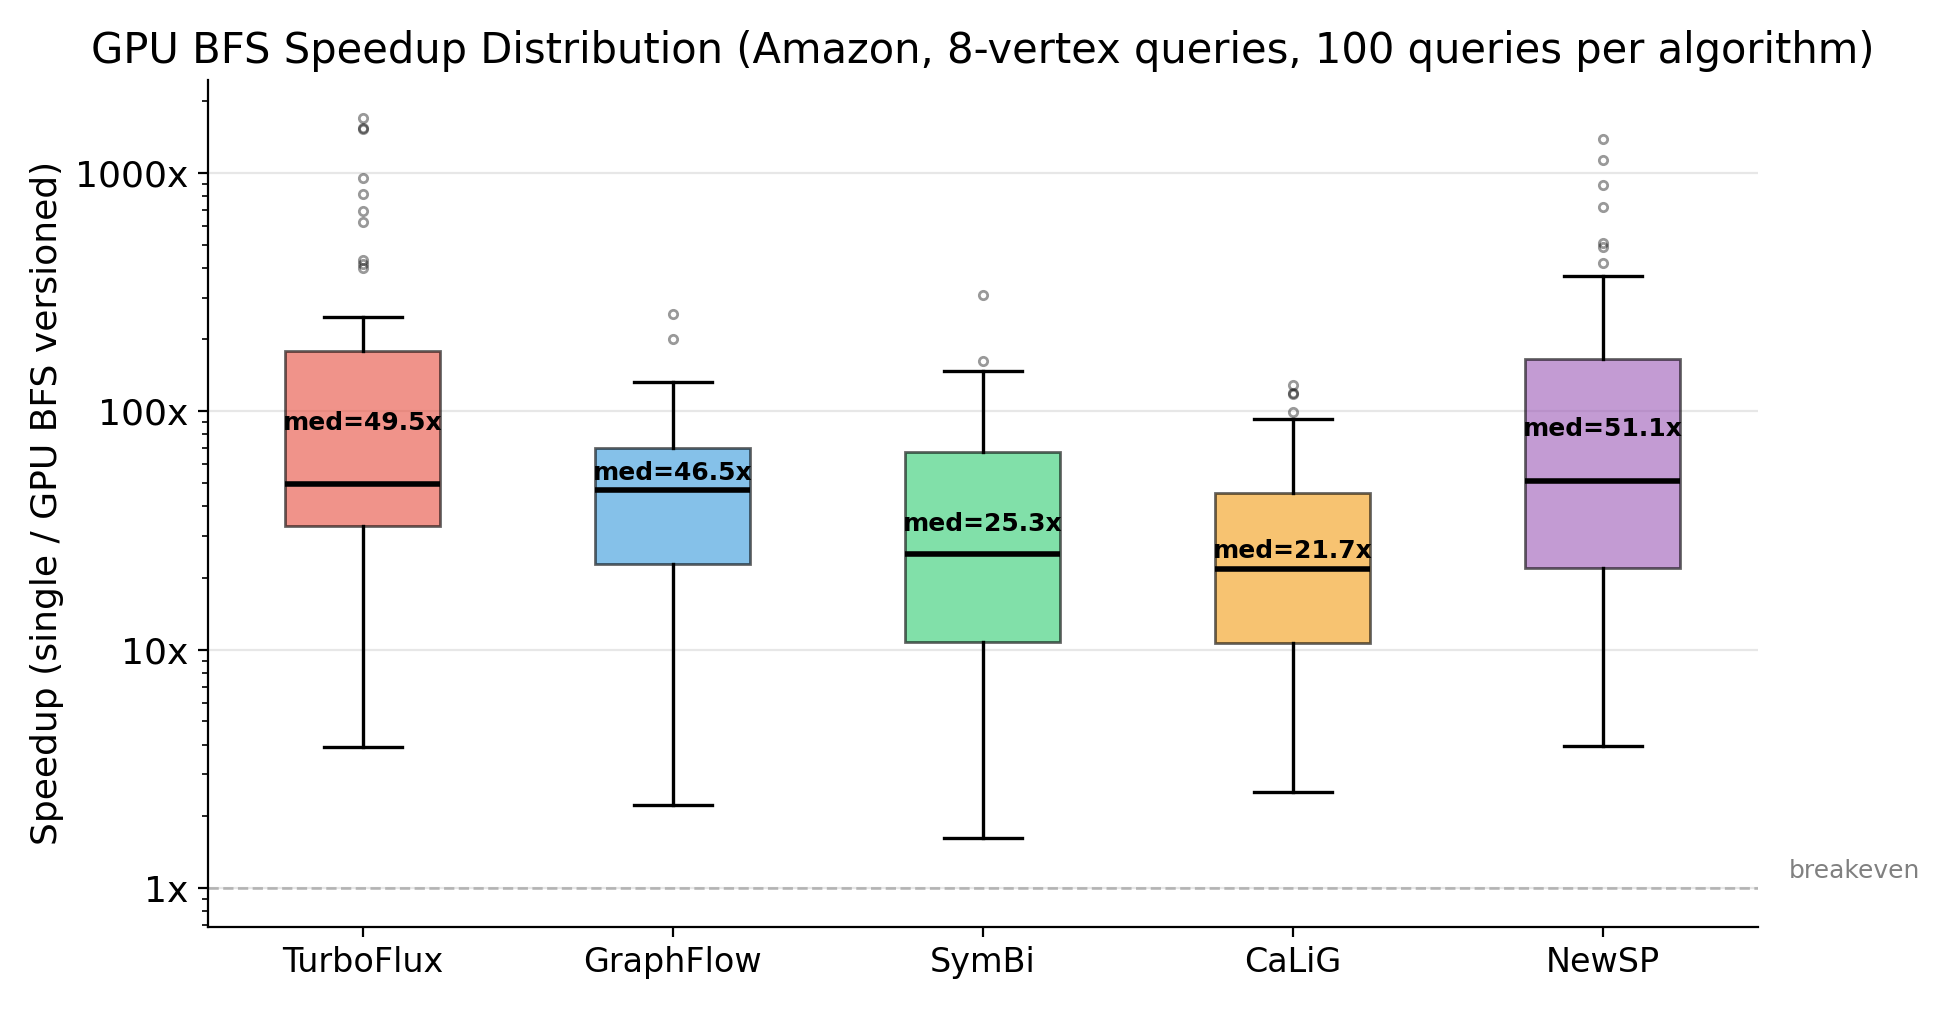
\includegraphics[width=\columnwidth]{figures/speedup_8v_by_algo.png}
  \caption{Median speedup of GPU \texttt{gpu\_bfs\_versioned} over CPU \texttt{single} on the AZ 8-vertex workload. Each box aggregates 100 queries. \textsc{NewSP} achieves the largest speedup; \textsc{CaLiG}, which already pays a heavy index cost on the CPU, achieves the smallest.}
  \label{fig:speedup-az}
\end{figure}

\begin{table}[t]
  \centering
  \small
  \caption{Per-algorithm median speedup on AZ 8v (100 queries each).}
  \label{tab:az-medians}
  \begin{tabular}{lr}
    \toprule
    \textbf{Algorithm} & \textbf{Median speedup} \\
    \midrule
    \textsc{Parallel\_NewSP}      & $51.1\times$ \\
    \textsc{Parallel\_TurboFlux}  & $49.5\times$ \\
    \textsc{Parallel\_GraphFlow}  & $46.5\times$ \\
    \textsc{Parallel\_SymBi}      & $25.3\times$ \\
    \textsc{Parallel\_CaLiG}      & $21.7\times$ \\
    \bottomrule
  \end{tabular}
\end{table}

\paragraph{Search-tree growth.}
The level-synchronous BFS makes the partial-match growth observable directly. Figure~\ref{fig:tree-q5} plots the count of partial matches at each depth for AZ \textsc{GraphFlow} \texttt{Q\_5}. The middle layers grow super-linearly and the final layer contracts as the last-vertex constraint kicks in. Crucially, the maximum partial-match count for AZ stays comfortably under the $4\times10^{8}$ device buffer and BFS proceeds without flushes.

\begin{figure}[t]
  \centering
  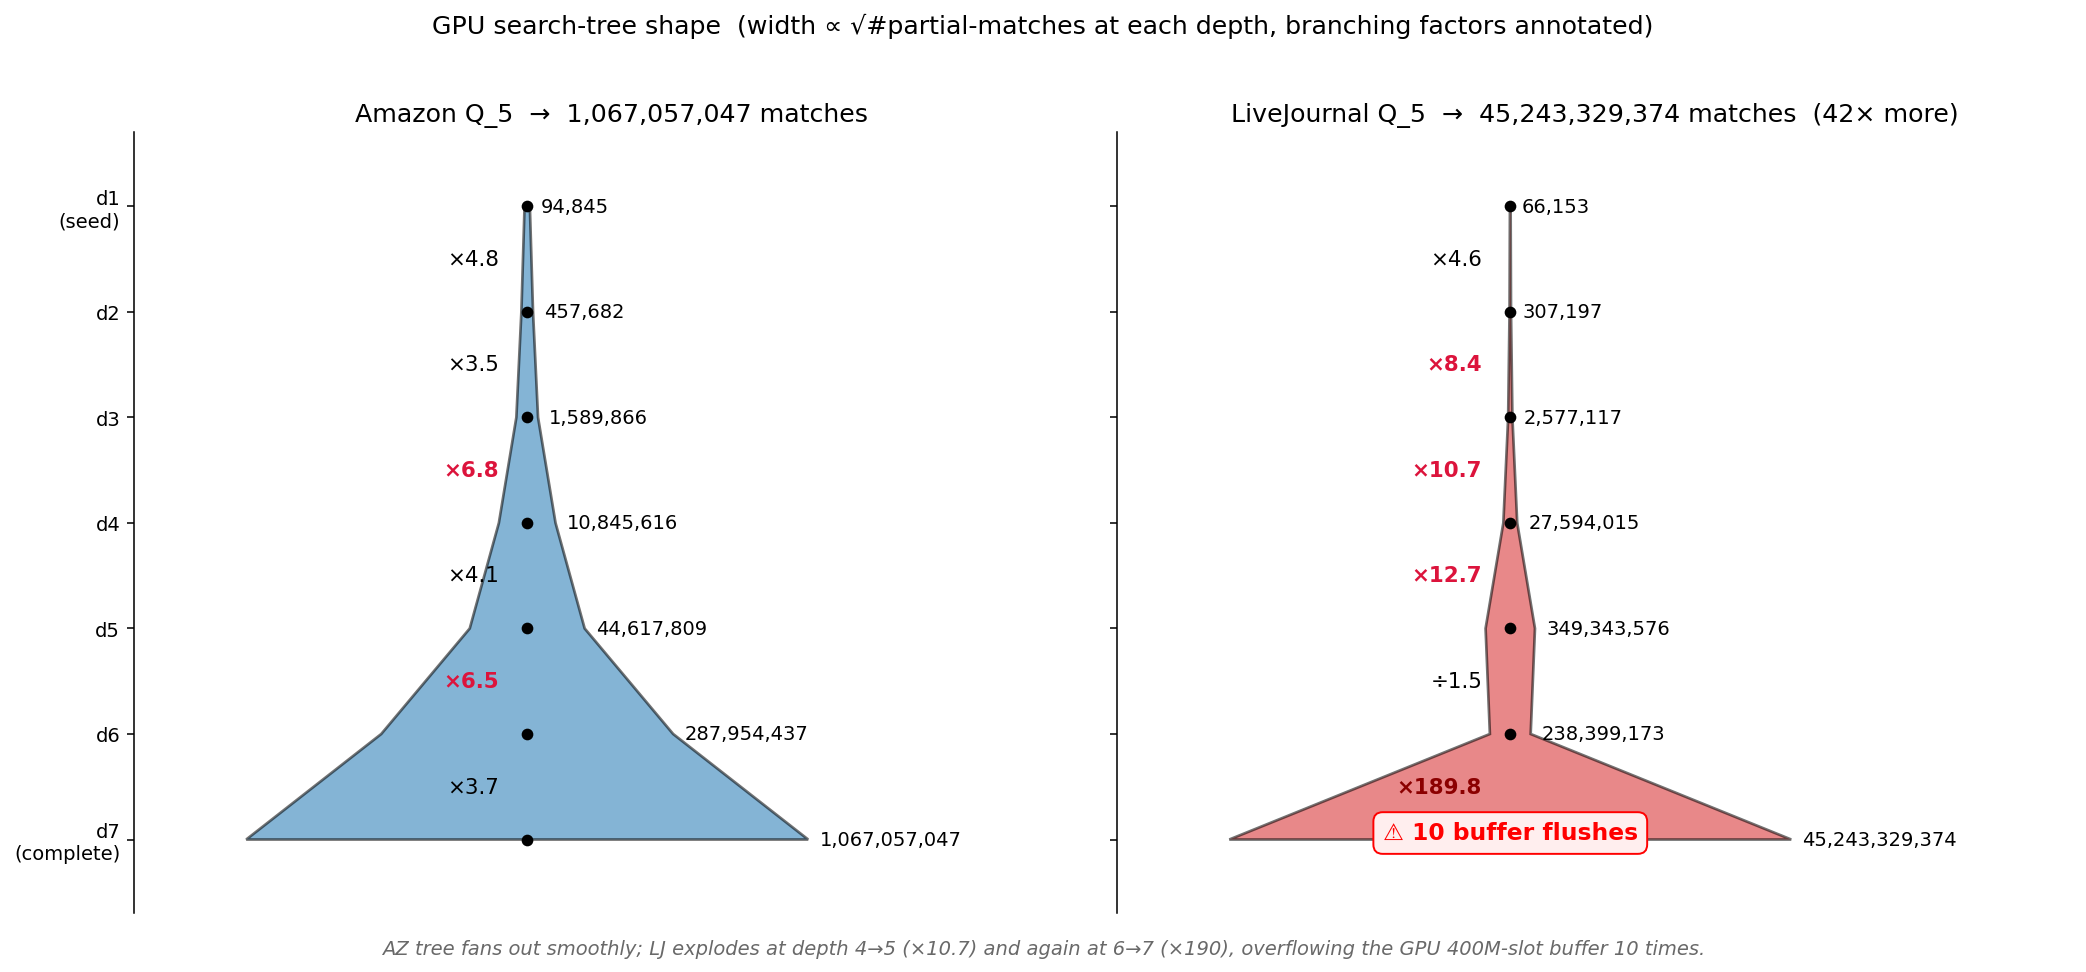
\includegraphics[width=\columnwidth]{figures/bfs_tree_q5_silhouette.png}
  \caption{BFS partial-match count by depth on AZ \textsc{GraphFlow} \texttt{Q\_5}. The middle expansion (depth 4--5) is the load-balancing-critical region. Final-depth contraction is induced by the last-vertex backward-neighbor constraint.}
  \label{fig:tree-q5}
\end{figure}

\paragraph{Best-case analysis.}
\textsc{NewSP} achieves $51\times$ on AZ because its CPU implementation re-runs a relatively expensive per-update search, while the GPU BFS amortizes both classification and partial-match expansion across the 4.3\,M-edge update stream. Kernel-time breakdown for a representative AZ \textsc{NewSP} query is dominated by the BFS search itself ($>90\%$); classification, edge insertion, and CSR build add up to under 10\%.

\paragraph{Worst-case analysis (within AZ).}
\textsc{CaLiG} achieves only $21.7\times$ because its CPU baseline already maintains a candidate-set index and short-circuits a large fraction of the search. The GPU still wins, but the absolute CPU time is small enough that PCIe + kernel-launch overhead becomes a non-trivial fixed cost.

% ============================================================================
\section{Boundary Case: Sparse, Skewed LiveJournal (LJ)}
% ============================================================================
\label{sec:lj}

We probe the boundary of GPU benefit on the LiveJournal graph: $|V|\approx 4.8$\,M, $|E|\approx 38.6$\,M, mean degree $\sim 16$, but with a heavy-tailed degree distribution.

\paragraph{Headline numbers.} On 20 sampled 8-vertex queries with 1800\,s time limits per algorithm-query pair, restricting to pairs where both CPU and GPU completed (Table~\ref{tab:lj}), the picture is mixed:

\begin{table}[t]
  \centering
  \small
  \caption{LJ 8v, restricted to queries where both CPU \texttt{single} and GPU \texttt{gpu\_bfs\_versioned} returned within 1800\,s. \textsc{NewSP} CPU is a stub on this code path, so its column is reported but not fair (see text).}
  \label{tab:lj}
  \begin{tabular}{lrrrr}
    \toprule
    \textbf{Algorithm} & \textbf{pairs} & \textbf{cpu\,(s)} & \textbf{gpu\,(s)} & \textbf{spd-up} \\
    \midrule
    \textsc{GraphFlow} &  1 & 1494.6 &  105.4 & $14.18\times$ \\
    \textsc{TurboFlux} &  9 &  666.3 &  215.2 & $3.10\times$  \\
    \textsc{CaLiG}     & 14 &  583.6 &  658.9 & $0.89\times$  \\
    \textsc{NewSP$^*$} & 16 &   87.1 &  637.0 & $0.14\times$  \\
    \textsc{SymBi}     &  0 & ---    & ---    & ---           \\
    \bottomrule
  \end{tabular}
\end{table}

Two observations stand out.

\paragraph{Search-space explosion and buffer flush.}
LJ \textsc{NewSP} \texttt{Q\_19} produces $7.97\times10^{10}$ matches, and the BFS frontier overflows the 400-million-entry partial-match buffer 15 times during the depth-6$\to$7 expansion. The corresponding log fragment is a clean diagnostic of the bottleneck:

\begin{small}
\begin{verbatim}
[BFS-V] Depth 5->6: 4.83e7 -> 3.85e8
[BFS-V] Flush 400000000 partials at depth 6->7  (x15)
Search complete: 7.97e10 matches, 1019.0 s
\end{verbatim}
\end{small}

Figure~\ref{fig:tree-az-vs-lj} shows the same level-by-level partial-match curves for AZ and LJ on the same query, on log scale; LJ's frontier is $\sim 10\times$ the AZ frontier at every depth and the device buffer is the binding constraint, not arithmetic throughput.

\begin{figure}[t]
  \centering
  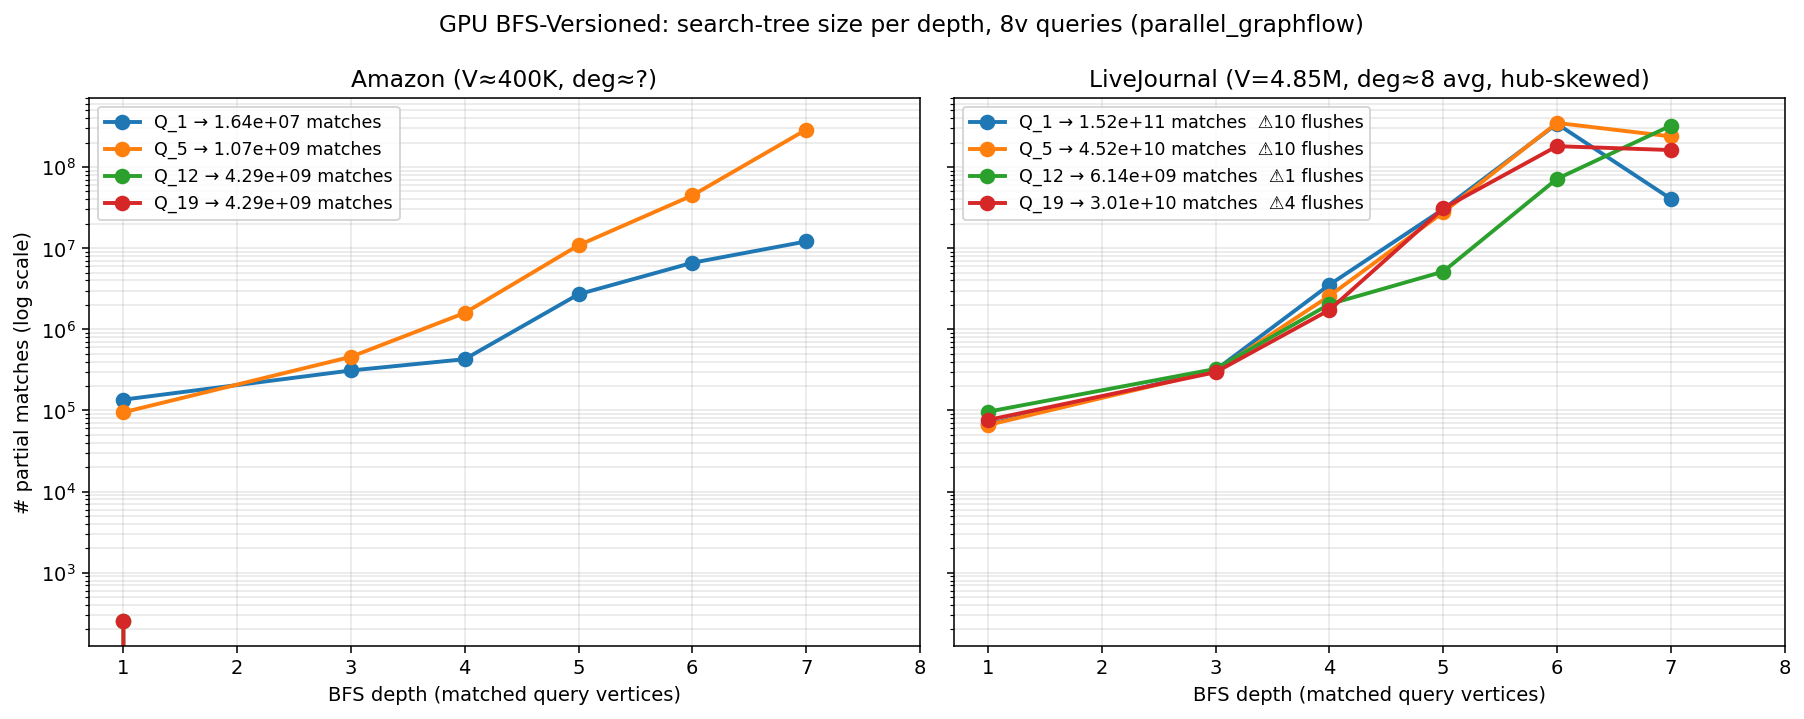
\includegraphics[width=\columnwidth]{figures/bfs_tree_az_vs_lj.png}
  \caption{Log-scale partial-match count by BFS depth: AZ vs LJ on a representative \textsc{GraphFlow} 8-vertex query. The LJ middle layers exceed the 400\,M-entry device buffer; LJ \textsc{NewSP} \texttt{Q\_19} flushes 15 times in the depth-6$\to$7 step.}
  \label{fig:tree-az-vs-lj}
\end{figure}

\paragraph{The \textsc{NewSP} CPU column is a stub.}
The CPU \texttt{single} mode for \textsc{NewSP} reports 0 positive matches on every LJ query, while GPU returns the expected $10^9$--$10^{10}$ counts. Inspecting \texttt{Parallel\_NewSP\_Adapter} explains why:

\begin{small}
\begin{verbatim}
size_t EnumerateNewEdge(uint v1, uint v2,
                        uint label, size_t /*tid*/) {
  // Not implemented for NewSP adapter -- use versioned mode
  return 0;
}
\end{verbatim}
\end{small}

The CPU \texttt{single} path therefore performs no actual matching for \textsc{NewSP}, which makes CPU look spuriously fast on LJ. A separate CPU \texttt{versioned} run (in progress at the time of writing) is the apples-to-apples comparison; the cross-validation on the four other algorithms (matching counts agree to seven significant digits between CPU and GPU) confirms that the BFS implementation itself is correct.

% ============================================================================
\section{Improvement Directions}
% ============================================================================
\label{sec:improvements-short}
We list improvements in order of expected return on engineering effort.

\paragraph{Short-term.}
\begin{itemize}
  \item \emph{Work-balanced BFS frontier.} Switch from one-thread-per-partial-match to edge-centric work split with block-binary-search, removing hub-vertex tail latency.
  \item \emph{Streaming partial matches.} When the device buffer is full, stream the overflow to host pinned memory under a CUDA stream so that the next BFS step proceeds in parallel with the H2D copy. This directly fixes the LJ flush-thrashing.
  \item \emph{H2D / search overlap.} Insert update batches via a dedicated stream so that subsequent BFS searches do not stall on edge insertion.
\end{itemize}

\paragraph{Medium-term.}
\begin{itemize}
  \item \emph{Adaptive DFS$\leftrightarrow$BFS.} For algorithm-query pairs where the candidate set is small enough that BFS launch overhead dominates, fall back to the DFS path; predicate the choice on a cost model that uses query topology and the first BFS-level candidate count.
  \item \emph{Early intersection pruning.} Apply the backward-neighbor intersection at partial-match emission time, not at the next BFS step; this is particularly valuable on skewed graphs like LJ where intermediate frontiers are dominated by partial matches that will be pruned at the next step.
\end{itemize}

\paragraph{Long-term.}
\begin{itemize}
  \item \emph{Multi-GPU.} Partition along the query axis (one GPU per query) for low-coupling workloads, or along the update axis for query-coupled workloads.
  \item \emph{CPU/GPU hybrid.} Route safe updates to CPU and unsafe to GPU; complete the missing CPU \texttt{versioned} implementations of \textsc{NewSP} so that the per-algorithm placement decision can be data-driven.
\end{itemize}

% ============================================================================
\section{Status and Reproducibility}
% ============================================================================
\label{sec:status}

\paragraph{Current status (as of writing).}
\begin{itemize}
  \item AZ 8v: complete on all five algorithms (100 queries each, 4 of 5 finished within the 1800\,s per-pair budget for $>95\%$ of queries).
  \item LJ 8v: 20 sampled queries; per-pair completion as reported in Table~\ref{tab:lj}. \textsc{SymBi} did not complete a single (CPU,\,GPU) pair within the time limit.
  \item Cross-validation: GPU and CPU \textsc{GraphFlow}/\textsc{TurboFlux}/\textsc{SymBi}/\textsc{CaLiG} match counts agree to seven significant digits where both finished, confirming the BFS implementation is correct.
  \item In-progress: a CPU \texttt{-m versioned} re-run for \textsc{NewSP} on LJ to replace the stub-affected CPU column in Table~\ref{tab:lj}.
\end{itemize}

\paragraph{Code and artifacts.}
All code, scripts, and raw logs are in the public ParaCOSM repository (\texttt{SUSTech-HPCLab/ParaCOSM}, branch \texttt{report}). The relevant locations are:

\begin{itemize}
  \item \texttt{ParaCOSM/CSM/}: GPU back-end (\texttt{matching\_executor/}, \texttt{graph\_storage/}) and the five algorithm adapters.
  \item \texttt{ParaCOSM/CSM/script\_bash/}: experiment drivers (one shell script per workload).
  \item \texttt{analysis/}: parsed run logs and aggregated CSVs feeding the figures in this report.
  \item \texttt{docs/gpu\_csm\_report/report/}: this paper, slides, and figure-generation notebooks; \texttt{make all} reproduces both PDFs.
\end{itemize}

\paragraph{Hardware.} Reproducing the exact wall-time numbers requires an A100-SXM4-80GB and a dual Xeon Platinum 8470 host; relative speedups should reproduce on any \texttt{sm\_80} or newer card with at least 40\,GB of device memory (the partial-match buffer alone consumes $\sim 32$\,GB).

% ============================================================================
\section{Conclusion}
% ============================================================================
We have shown that GPU acceleration of CSM is best framed as a level-synchronous BFS pipeline that consolidates the per-update search at fixed depth, rather than as a parallelized DFS. Four take-aways summarize the report:

\begin{enumerate}
  \item \textbf{BFS dominates DFS on the GPU.} On every algorithm-query pair we tried, \texttt{gpu\_bfs\_versioned} beats \texttt{gpu\_all}; the SIMT-level arguments of \S\ref{sec:bfs-vs-dfs} are matched by the empirical record.
  \item \textbf{Large speedups are real and algorithm-spanning.} On AZ 8v, BFS-versioned achieves $21\times$--$51\times$ median speedup over a tuned single-thread CPU baseline across all five state-of-the-art CSM systems, not just one.
  \item \textbf{The boundary failure mode is identifiable.} On LJ the BFS frontier overflows the fixed-size device buffer and the run becomes H2D-flush bound rather than arithmetic-bound; each short-term improvement in \S\ref{sec:improvements-short} (or its surrounding section) targets a directly measured bottleneck.
  \item \textbf{Level-by-level partial-match profiling is portable.} Tracking the size of the BFS frontier at every depth, as in Figs.~\ref{fig:tree-q5} and~\ref{fig:tree-az-vs-lj}, generalizes beyond CSM to any GPU graph-mining workload that fits a level-synchronous pattern.
\end{enumerate}

\bibliographystyle{plain}
\bibliography{report}

\end{document}
